\section{Excess velocity at arrival}

The excess velocity at arrival is the difference between the velocity of the
spacecraft and the velocity of the interloper at arrival. The
velocity of the spacecraft at arrival is denoted by $\vec{v_{\infty ,2}}$. Note
that this velocity represents the velocity after the second impulse of Lambert's
maneuver, leading to a rendezvous with the interloper. The velocity of the
interloper at arrival is $\vec{v_\text{ISO}}$. Thus, the excess velocity at
arrival is:

\begin{equation}
  \Delta v_2 = \norm{\vec{v_{\infty ,2}} - \vec{v_\text{ISO}}}
\end{equation}

As discussed in subsection \ref{sec:excess_velocity}, applying this last impulse
can be avoided on behalf performing a targeting mission. This allows to allocate
more $\Delta v$ for the first impulse.

\subsection{'Oumuamua}

Porkchop plots for 1I/'Oumuamua representing the excess velocity at arrival are
shown in figure \ref{fig:oumuamua-direct-prograde-transfer-porkchop-avl} and figure
\ref{fig:oumuamua-direct-retrograde-transfer-porkchop-avl}.

For short-duration flights, the velocity surplus upon arrival is notably higher,
contrasting with longer flights where the surplus is reduced. Both prograde and
retrograde transfers exhibit a similar trend in arrival velocity.

Interestingly, the isolines depicting excess arrival velocity reveal a
distinctive pattern, all originating from a shared point circa late 2017 for
both launch and arrival.

Of particular significance is the area delineated by the $2.0$ km/s isoline in
prograde transfers, representing an optimal velocity for rendezvous with the
interloper given current technological capabilities. Examining the
time-of-flight data in Figure
\ref{fig:oumuamua-direct-prograde-transfer-porkchop}, this region necessitates a
minimum trip duration of at least 5 years. It is worth noting that the only
constraints on flight duration are those dictated by mission requirements.

\newpage
\begin{figure}[H]
  \centering
  \includegraphics[width=\textwidth]{static/oumuamua/direct-prograde-transfer-porkchop-avl.png}
  \caption[Direct and prograde launch energy porkchop for 'Oumuamua]{Launch energy porkchop plot for 1I/'Oumuamua for a direct and prograde transfer showing the isolines for the arrival velocity required for a rendezvous.}
  \label{fig:oumuamua-direct-prograde-transfer-porkchop-avl}
\end{figure}

\begin{figure}[H]
  \centering
  \includegraphics[width=\textwidth]{static/oumuamua/direct-retrograde-transfer-porkchop-avl.png}
  \caption[Direct and prograde launch energy porkchop for
    'Oumuamua]{Launch energy porkchop plot for 1I/'Oumuamua for a direct and
    retrograde transfer showing the isolines for the arrival velocity required for a rendezvous.}
  \label{fig:oumuamua-direct-retrograde-transfer-porkchop-avl}
\end{figure}

\subsection{Borisov}

Porkchop plots for 2I/Borisov representing the excess velocity at arrival are
shown in figures \ref{fig:borisov-direct-prograde-transfer-porkchop-avl} and
\ref{fig:borisov-direct-retrograde-transfer-porkchop-avl}.

\begin{figure}[H]
  \centering
  \includegraphics[width=\textwidth]{static/borisov/direct-prograde-transfer-porkchop-avl.png}
  \caption[Direct and prograde arrival excess velocity porkchop for
    Borisov]{Launch energy porkchop plot for 2I/Borisov for a direct and
    prograde transfer showing the isolines for excess velocity at arrival
    for a rendezvous.}
  \label{fig:borisov-direct-prograde-transfer-porkchop-avl}
\end{figure}

\begin{figure}[H]
  \centering
  \includegraphics[width=\textwidth]{static/borisov/direct-retrograde-transfer-porkchop-avl.png}
  \caption[Direct and retrograde arrival excess velocity porkchop for
    Borisov]{Launch energy porkchop plot for 2I/Borisov for a direct and
    retrograde transfer showing the isolines for excess velocity at arrival
    for a rendezvous.}
  \label{fig:borisov-direct-retrograde-transfer-porkchop-avl}
\end{figure}

Once again, the excess velocity at arrival for Borisov remembers the ones for
the case of 'Oumuamua. Again, the values are different and higher for the second
discovered interloper.

Similarly to 'Oumuamua, the lines for the arrival velocity start at a common
point. In this case, the point is located at the beginning of 2020 for launch
dates. However, the main difference with the first discovered interloper is that
a series of closed lines shows for an arrival at year 2020. This could indicate
a periodic solution. This region is analyzed in detail in the next section.
